\chapter{AP-Regelung Systemparametertests}

\newcommand{\scalea}{0.62}
\begin{figure}[h]
	\centering
	\subfloat[\apaz]{ \includegraphics[scale=\scalea]{Bilder/SysParam Variation/m0/AP2.pdf}	}
	\hfil
	\subfloat[\apad]{	\includegraphics[scale=\scalea]{Bilder/SysParam Variation/m0/AP3.pdf}	}
	\\
	\subfloat[\apave]{ \includegraphics[scale=\scalea]{Bilder/SysParam Variation/m0/AP41.pdf} }
	\hfil
	\subfloat[\apavz]{ \includegraphics[scale=\scalea]{Bilder/SysParam Variation/m0/AP42.pdf}	}
	\caption{Maximale Startwerte -- Variation $m_0$}
	\label{fig:sysvarm0}
\end{figure}

\renewcommand{\scalea}{0.38}
\begin{figure}[h]
	\centering
	\subfloat[\apaz]{ \includegraphics[scale=\scalea]{Bilder/SysParam Variation/s1/AP2.pdf}	}
	%\hfil
	\subfloat[\apad]{	\includegraphics[scale=\scalea]{Bilder/SysParam Variation/s1/AP3.pdf}	}
	\\
	\subfloat[\apave]{ \includegraphics[scale=\scalea]{Bilder/SysParam Variation/s1/AP41.pdf} }
	%\hfil
	\subfloat[\apavz]{ \includegraphics[scale=\scalea]{Bilder/SysParam Variation/s1/AP42.pdf}	}
	\caption{Maximale Startwerte -- Variation $s_1$}
	\label{fig:sysvars1}
\end{figure}

\begin{figure}
	\centering
	\subfloat[\apaz]{ \includegraphics[scale=\scalea]{Bilder/SysParam Variation/s2/AP2.pdf}	}
	%\hfil
	\subfloat[\apad]{	\includegraphics[scale=\scalea]{Bilder/SysParam Variation/s2/AP3.pdf}	}
	\\
	\subfloat[\apave]{ \includegraphics[scale=\scalea]{Bilder/SysParam Variation/s2/AP41.pdf} }
	%\hfil
	\subfloat[\apavz]{ \includegraphics[scale=\scalea]{Bilder/SysParam Variation/s2/AP42.pdf}	}
	\caption{Maximale Startwerte -- Variation $s_2$}
	\label{fig:sysvars2}
\end{figure}

\begin{figure}
	\centering
	\subfloat[\apaz]{ \includegraphics[scale=\scalea]{Bilder/SysParam Variation/l1/AP2.pdf}	}
	%\hfil
	\subfloat[\apad]{	\includegraphics[scale=\scalea]{Bilder/SysParam Variation/l1/AP3.pdf}	}
	\\
	\subfloat[\apave]{ \includegraphics[scale=\scalea]{Bilder/SysParam Variation/l1/AP41.pdf} }
	%\hfil
	\subfloat[\apavz]{ \includegraphics[scale=\scalea]{Bilder/SysParam Variation/l1/AP42.pdf}	}
	\caption{Maximale Startwerte -- Variation $l_1$}
	\label{fig:sysvarl1}
\end{figure}